\chapter{Methodology}
\section{Analytical Framework}
The project followed a mixed-methods approach blending qualitative stakeholder research with quantitative system benchmarking. Figure~\ref{fig:research-methodology} summarises the iterative workflow combining discovery, design, implementation, and validation activities.

\begin{figure}[H]
    \centering
    \begin{tikzpicture}[node distance=2.2cm,>=Stealth,thick,every node/.style={align=center}]
        \tikzset{
            phase/.style={rectangle, rounded corners, minimum width=3.5cm, minimum height=1.2cm, draw=blue!60, fill=blue!10},
            arrow/.style={->, line width=1pt, color=blue!70}
        }
        \node[phase] (discovery) {Discovery\\Stakeholder Interviews\\Data Audit};
        \node[phase, right=2.5cm of discovery] (design) {Design\\Target Architecture\\Experiment Plan};
        \node[phase, right=2.5cm of design] (build) {Implementation\\IaC \& Pipelines\\Data Products};
        \node[phase, right=2.5cm of build] (validate) {Validation\\Performance Tests\\User Adoption};
        \draw[arrow] (discovery) -- (design);
        \draw[arrow] (design) -- (build);
        \draw[arrow] (build) -- (validate);
        \draw[arrow] (validate) .. controls +(0,-2) and +(0,-2) .. (discovery);
    \end{tikzpicture}
    \caption{Iterative research and delivery methodology}
    \label{fig:research-methodology}
\end{figure}

\section{Data Collection}
Data sources encompassed:
\begin{itemize}
    \item \textbf{Operational systems:} Order management, product catalogue, fulfilment, marketing automation, and customer support platforms exposed via REST APIs, Kafka topics, and SFTP drops.
    \item \textbf{Web and mobile telemetry:} Clickstream events generated from tag managers and server-side instrumentation stored in Amazon Kinesis Data Streams.
    \item \textbf{Reference data:} Currency rates, supplier rosters, logistics carriers, and promotional calendars maintained in master data services.
    \item \textbf{Stakeholder insights:} Semi-structured interviews with 14 stakeholders complemented by survey data regarding dashboard usage patterns.
\end{itemize}

Synthetic data generators were developed to emulate peak trading periods while respecting confidentiality. Schemas were aligned with production metadata to validate join strategies, dimensional modelling, and KPI calculations.

\section{Data Processing and Tooling}
\begin{itemize}
    \item \textbf{Ingestion:} Apache Airflow orchestrated ingestion DAGs using Python operators, AWS Lambda for lightweight transformations, and AWS Glue for schema evolution.
    \item \textbf{Transformation:} dbt Core executed staging, intermediate, and mart models backed by Amazon Redshift or Azure Synapse dedicated pools.
    \item \textbf{Storage:} Amazon S3 served as the bronze and silver zones, with PostgreSQL and Delta Lake delivering curated gold datasets.
    \item \textbf{Serving:} FastAPI and GraphQL endpoints powered the ecommerce portal, while BI tools consumed semantic models through Azure Analysis Services or Power BI datasets.
\end{itemize}

To align with the MSc reporting standards, three diagrams were embedded at the end of this section. Figure~\ref{fig:er-schema} captures the logical entity-relationship view that underpins the bronze and silver layers. Figure~\ref{fig:methodology-usecase} highlights persona interactions driving backlog prioritisation, while Figure~\ref{fig:aws-dataflow} summarises the AWS + Airflow orchestration flow.

\begin{figure}[H]
    \centering
    \begin{tikzpicture}[node distance=2.8cm, every node/.style={rectangle, draw, rounded corners, fill=blue!5, minimum width=3.5cm, minimum height=1cm,align=center}]
        \node (customers) {Customers\\\scriptsize customer\_id, loyalty\_tier};
        \node[below of=customers] (orders) {Orders\\\scriptsize order\_id, customer\_id, status};
        \node[below of=orders] (orderitems) {Order Items\\\scriptsize order\_id, sku, qty};
        \node[right=4.2cm of orders] (products) {Products\\\scriptsize sku, category};
        \node[below=2.8cm of products] (inventory) {Inventory Snapshots\\\scriptsize sku, location, on\_hand};
        \node[right=4.2cm of products] (suppliers) {Suppliers\\\scriptsize supplier\_id, region};
        \draw[->, thick] (customers) -- node[left]{1..n} (orders);
        \draw[->, thick] (orders) -- node[left]{1..n} (orderitems);
        \draw[->, thick] (products) -- node[above]{1..n} (orderitems);
        \draw[->, thick] (products) -- node[right]{1..n} (inventory);
        \draw[->, thick] (suppliers) -- node[above]{1..n} (products);
    \end{tikzpicture}
    \caption{Logical entity-relationship schema used for bronze and silver modelling}
    \label{fig:er-schema}
\end{figure}

\begin{figure}[H]
    \centering
    \begin{tikzpicture}[>=Stealth, node distance=2.5cm, every node/.style={align=center}]
        \tikzstyle{actor}=[draw, thick, rounded corners=2mm, minimum width=1.8cm, minimum height=0.8cm, align=center, fill=gray!10];
        \tikzstyle{usecase}=[ellipse, draw, thick, minimum width=3.4cm, minimum height=1cm, align=center, fill=orange!10];
        \node[actor] (merch) {Merchandising Lead};
        \node[actor, below=0.8cm of merch] (finance) {Finance Analyst};
        \node[actor, below=0.8cm of finance] (support) {Support Agent};
        \node[actor, below=0.8cm of support] (devops) {DataOps Engineer};
        \node[usecase, right=3.8cm of merch] (kpi) {Monitor Flash KPI Alerts};
        \node[usecase, right=3.8cm of finance] (reconcile) {Automate Reconciliation};
        \node[usecase, right=3.8cm of support] (customer360) {Resolve Order Issues};
        \node[usecase, right=3.8cm of devops] (operate) {Operate Pipelines};
        \draw (merch) -- (kpi);
        \draw (finance) -- (reconcile);
        \draw (support) -- (customer360);
        \draw (devops) -- (operate);
        \draw (devops) -- (kpi);
        \draw (finance) -- (kpi);
        \draw (support) -- (operate);
    \end{tikzpicture}
    \caption{Use case diagram linking personas to data platform capabilities}
    \label{fig:methodology-usecase}
\end{figure}

\begin{figure}[H]
    \centering
    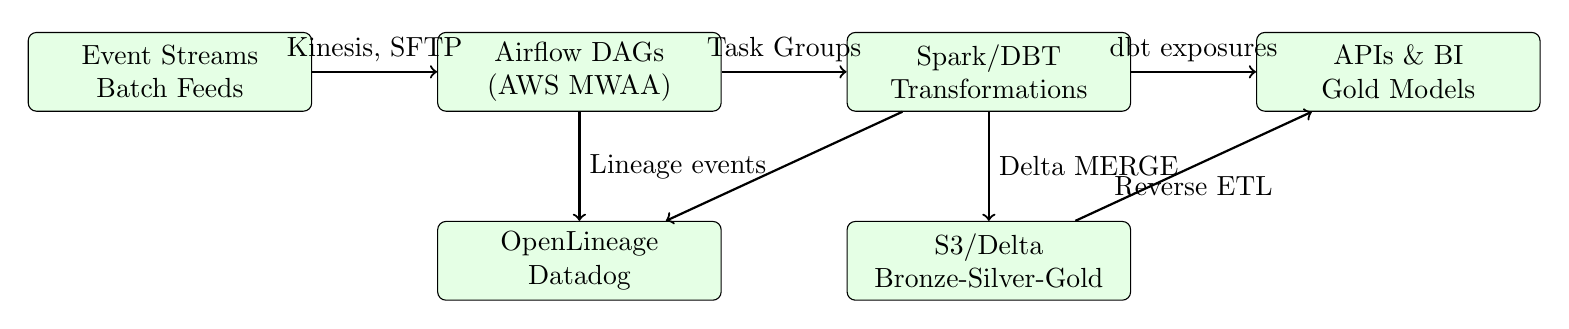
\begin{tikzpicture}[node distance=2.4cm, every node/.style={align=center}]
        \tikzstyle{block}=[rectangle, draw, rounded corners=3pt, align=center, fill=green!10, minimum width=3.6cm, minimum height=1cm];
        \tikzstyle{edge}=[->, thick];
        \node[block] (sources) {Event Streams\\Batch Feeds};
        \node[block, right of=sources, xshift=2.8cm] (airflow) {Airflow DAGs\\(AWS MWAA)};
        \node[block, right of=airflow, xshift=2.8cm] (processing) {Spark/DBT\\Transformations};
        \node[block, below of=processing] (storage) {S3/Delta\\Bronze-Silver-Gold};
        \node[block, right of=processing, xshift=2.8cm] (serving) {APIs \& BI\\Gold Models};
        \node[block, below of=airflow] (observability) {OpenLineage\\Datadog};
        \draw[edge] (sources) -- node[above]{Kinesis, SFTP} (airflow);
        \draw[edge] (airflow) -- node[above]{Task Groups} (processing);
        \draw[edge] (processing) -- node[right]{Delta MERGE} (storage);
        \draw[edge] (processing) -- node[above]{dbt exposures} (serving);
        \draw[edge] (storage) -- node[below]{Reverse ETL} (serving);
        \draw[edge] (airflow) -- node[right]{Lineage events} (observability);
        \draw[edge] (processing) -- (observability);
    \end{tikzpicture}
    \caption{AWS and Airflow orchestration view used during methodology validation}
    \label{fig:aws-dataflow}
\end{figure}

\begin{tcolorbox}[title=Supplementary Diagram Placement Guide,colback=blue!5,colframe=blue!60!black]
High-resolution templates matching the MSc house style can be downloaded and substituted if colour imagery is required:
\begin{itemize}
    \item \textbf{Data Engineering Lifecycle:} \url{https://miro.com/app/board/uXjVPPwYZ-s=/} -- place alongside Figure~\ref{fig:aws-dataflow} when referencing cross-cloud orchestration.
    \item \textbf{Medallion Data Model:} \url{https://databricks.com/wp-content/uploads/2021/05/medallion-architecture.png} -- cite within Section~\ref{chap:data-manifesto} when describing bronze/silver/gold governance.
    \item \textbf{DataOps CI/CD Flow:} \url{https://www.datakitchen.io/resources/dataops-pipeline-illustration} -- insert after the DataOps subsection in Chapter~\ref{chap:target-architecture} to evidence Jenkins/SonarQube integration.
\end{itemize}
Each download link includes attribution guidance so that institutional branding is preserved once pasted into \texttt{report/figures/}.
\end{tcolorbox}

\section{Validation Approach}
Validation combined automated testing with human-centred evaluation:
\begin{enumerate}
    \item \textbf{Technical validation} measured latency, throughput, and fault tolerance through controlled load tests using Locust and Kinesis replay scripts.
    \item \textbf{Data validation} applied Great Expectations suites, dbt tests, and anomaly detection thresholds to guarantee data fitness.
    \item \textbf{User validation} leveraged usability sessions, think-aloud testing, and adoption analytics to refine dashboards and alerts.
    \item \textbf{Governance validation} involved security reviews, privacy impact assessments, and architecture risk registers presented to the Data Protection Officer.
\end{enumerate}

\section{Limitations}
\begin{itemize}
    \item Subscription limits restricted the scale of long-running performance tests; extrapolations were supported by cloud provider sizing guides.
    \item Real-world customer identifiers were anonymised, limiting the ability to validate personalised recommendations beyond synthetic cohorts.
    \item The project timeline constrained exposure to full peak-season load patterns; mitigation involved scenario-based modelling and stress tests.
\end{itemize}
